\documentclass[10pt,twoside,english,a4paper]{article}
\usepackage[utf8]{inputenc}
\usepackage{graphicx}
\usepackage{url} 
\usepackage{hyperref} 
\usepackage{cite}
%\usepackage{times}
\pagestyle{headings}

\title{Improving computer science and software 
engineering education in cyberlearning 
environments through understanding UI and UX design
\thanks{Semestrálny projekt v predmete Metódy inžinierskej práce,
 ak. rok 2020/21, vedenie: Martin Sabo}}

\author{Márk Bartalos \\[2pt]
        \small{Slovak University of Technology in Bratislava}\\
        \small{Faculty of Informatics and Information Technologies}\\
        \small{\texttt{xbartalosm@stuba.sk}}
}

% \date{\small 30. september 2020}


\begin{document}

\maketitle

\begin{abstract}
    In our day and age cyberlearning for computer science and software engineering education has become more popular than ever. 
The article will be about how understanding UI and UX design principles can serve as a basis for future improvements in teaching
these fields. My goal is to understand UI/UX design techniques to be able to identify the problems with currently 
implemented cyberlearning environment designs. The identified problems then could be used to improve already existing environments.
Knowledge of these problems would be greatly beneficial in the design and development of new, learning focused, student 
oriented cyberlearning environments for computer science (CS) and software engineering (SE) students.
\end{abstract}



\section{Introduction}
We speak about distance learning from around two centuries ago\cite{moore_2011_elearning}, but only now
it is becoming a neccesity rather than an option. Especially now in the middle of a pandemic, use of online 
education environments is more needed than ever. This article will focus on online cyberlearning environments 
mainly designed for computer science and software engineer students. Implementing cyberlearning 
environments for teaching these fields can be the more beneficial than implementing it in teaching for non computer 
related fields. Design of the environment has a very big role in the effectiveness and in 
its ability to properly convey information. 
About the most common problems with the currently running cyberlearning environment (CLE)
designs I will talk about more in the following section.
The used methods which will be explored more in section *put section number here*.

\section{Definitions}

\subsection{Cyberlearning}
For cyberlearning I will use the definition by National Science Foundation: 
``the use of networked computing and communications technologies to support learning” \cite{borgman_2017_fostering} 
Cyberlearning itself is a form of distance learning, but its main focus is building an all 
encompassing online environment which can motivate, inspire and and teach students using 
computer systems and networking technologies as primary tools. \cite{ui/ux}
Primary goal of cyberlearning is to provide learning experiences via a technology-based platform. 
Cyberlearning in some way is an extension of e-learning and a form of distance learning.\cite{ui/ux}
It is a complete platform for learning instead of a method. 

\subsection{Cyberlearning env. for CS and SE students}
Under the term ``Cyberlearning environments for computer science and software engineer students', I am mainly
referring to those online CLE which enable students to write and compile code online. Using these CLEs 
students are able to learn the curriculum through lectures and through practice.




% Motivujte čitateľa a vysvetlite, o čom píšete. Úvod sa väčšinou nedelí na časti.

% Uveďte explicitne štruktúru článku. Tu je nejaký príklad.
% Základný problém, ktorý bol naznačený v úvode, je podrobnejšie vysvetlený v časti~\ref{nejaka}.
% Dôležité súvislosti sú uvedené v častiach~\ref{dolezita} a~\ref{dolezitejsia}.
% Záverečné poznámky prináša časť~\ref{zaver}.


\begin{figure}
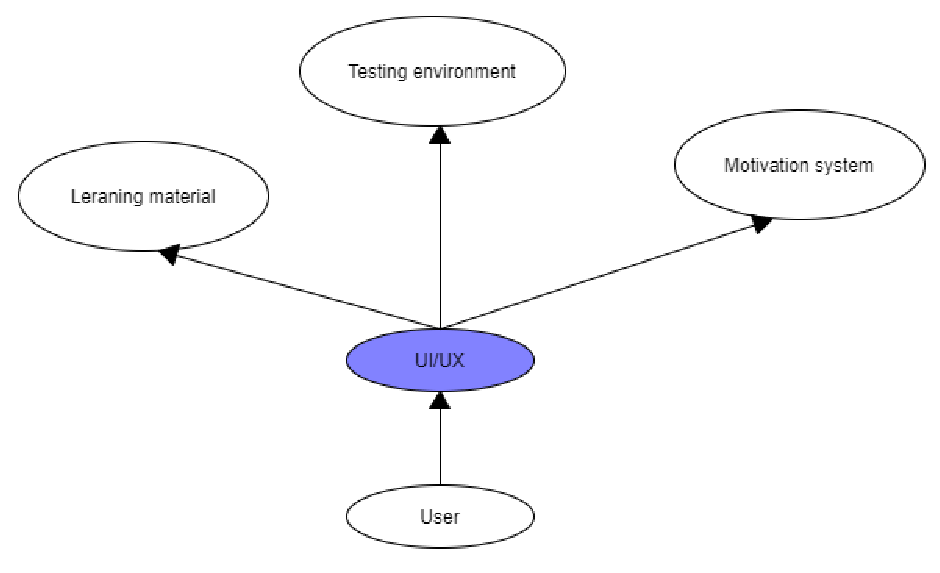
\includegraphics[width=0.75\textwidth]{images/diagram-crop.pdf}
\end{figure}

\begin{figure}
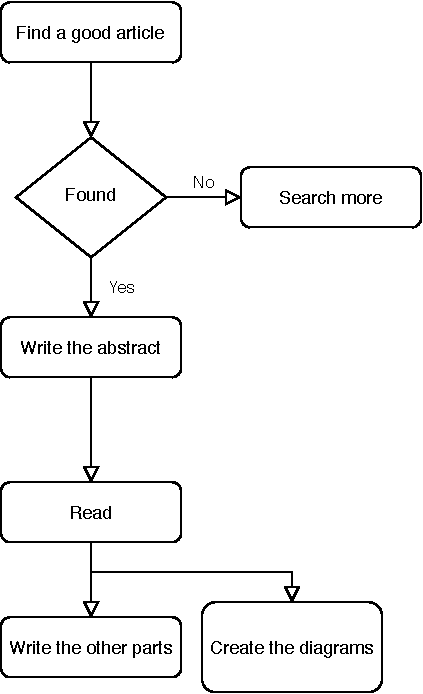
\includegraphics[width=0.75\textwidth]{images/flowchart-crop.pdf}
\end{figure}
% \section{Nejaká časť} \label{nejaka}

% Z obr.~\ref{f:rozhod} je všetko jasné. 

% \begin{figure*}[tbh]
% \centering
% %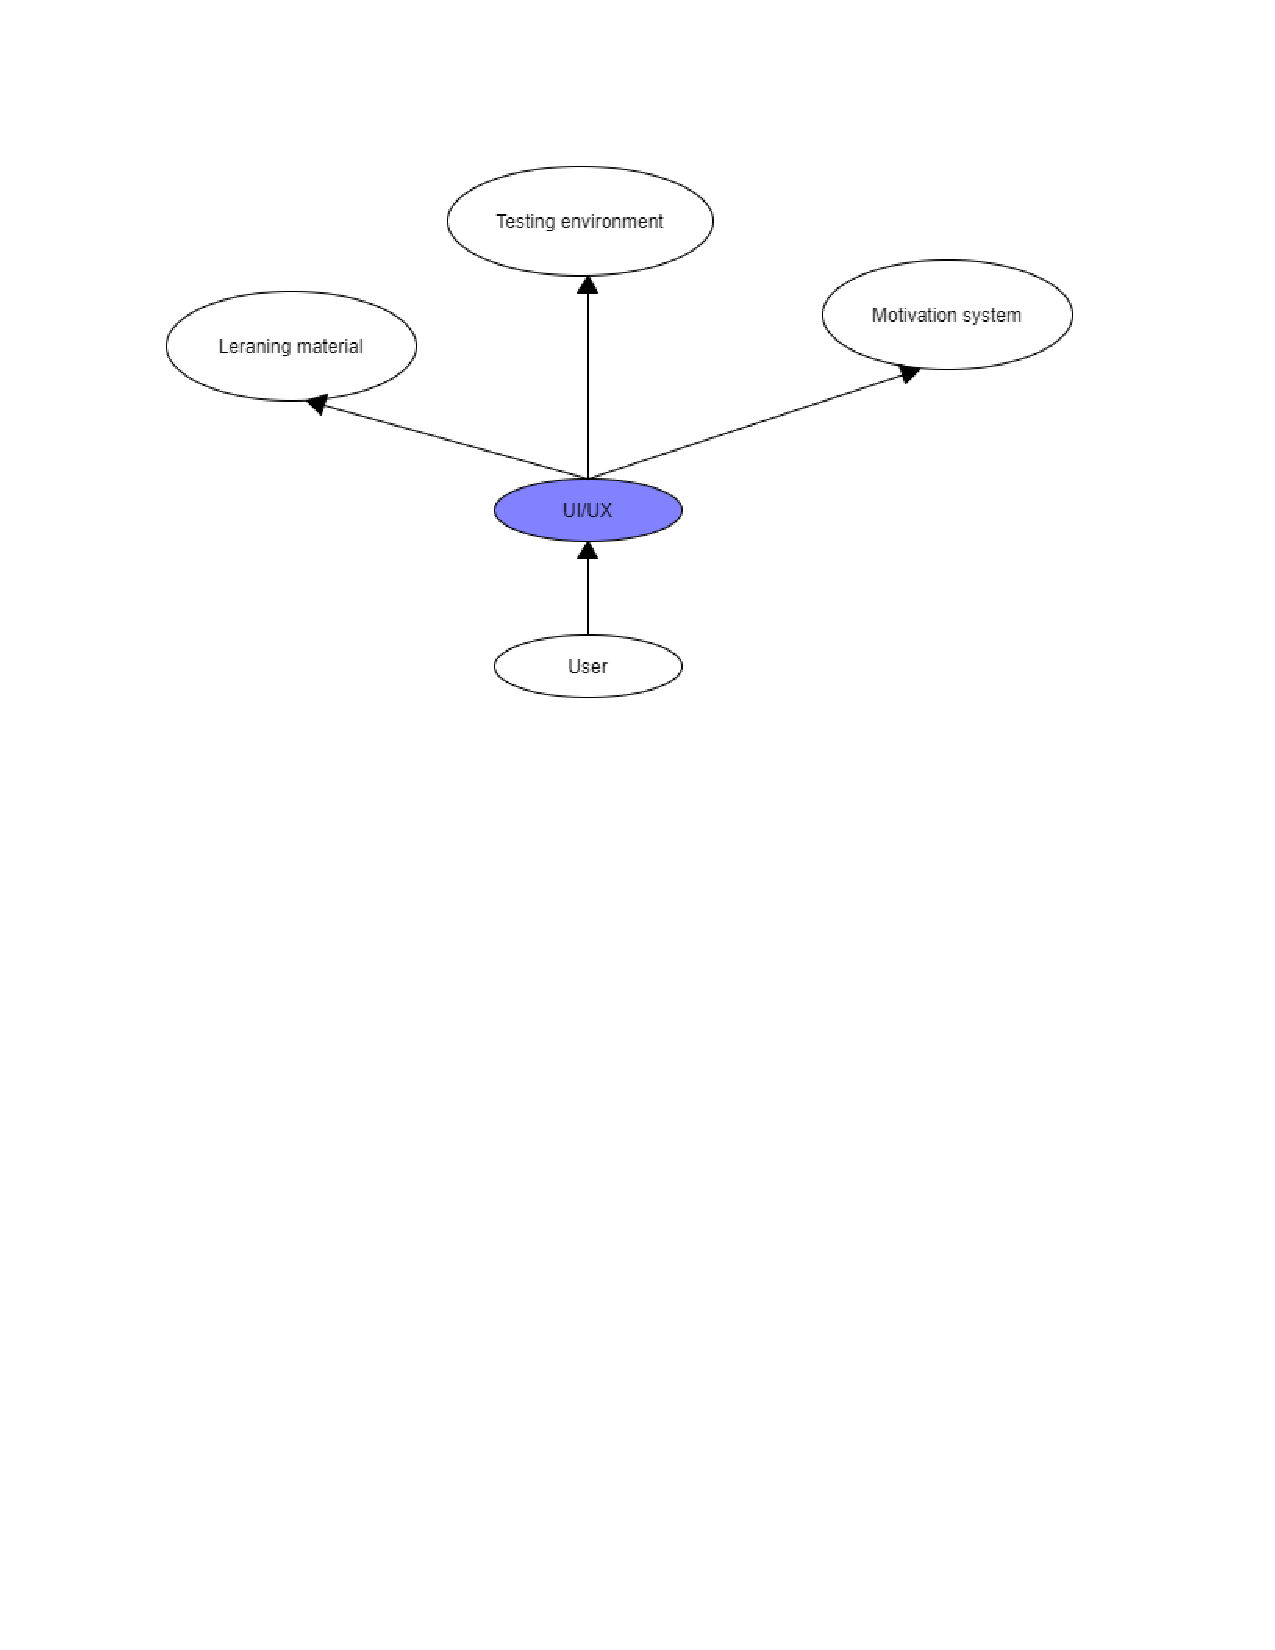
\includegraphics[scale=1.0]{diagram.pdf}
% Aj text môže byť prezentovaný ako obrázok. Stane sa z neho označný plávajúci objekt. Po vytvorení diagramu zrušte znak \texttt{\%} pred príkazom \verb|\includegraphics| označte tento riadok ako komentár (tiež pomocou znaku \texttt{\%}).
% \caption{Rozhodujúci argument.}
% \label{f:rozhod}
% \end{figure*}



% \section{Iná časť} \label{ina}

% Základným problémom je teda\ldots{} Najprv sa pozrieme na nejaké vysvetlenie (časť~\ref{ina:nejake}), a potom na ešte nejaké (časť~\ref{ina:nejake}).\footnote{Niekedy môžete potrebovať aj poznámku pod čiarou.}

% Môže sa zdať, že problém vlastne nejestvuje\cite{Coplien:MPD}, ale bolo dokázané, že to tak nie je~\cite{Czarnecki:Staged, Czarnecki:Progress}. Napriek tomu, aj dnes na webe narazíme na všelijaké pochybné názory\cite{PLP-Framework}. Dôležité veci možno \emph{zdôrazniť kurzívou}.


% \subsection{Nejaké vysvetlenie} \label{ina:nejake}

% Niekedy treba uviesť zoznam:

% \begin{itemize}
% \item jedna vec
% \item druhá vec
% 	\begin{itemize}
% 	\item x
% 	\item y
% 	\end{itemize}
% \end{itemize}

% Ten istý zoznam, len číslovaný:

% \begin{enumerate}
% \item jedna vec
% \item druhá vec
% 	\begin{enumerate}
% 	\item x
% 	\item y
% 	\end{enumerate}
% \end{enumerate}


% \subsection{Ešte nejaké vysvetlenie} \label{ina:este}

% \paragraph{Veľmi dôležitá poznámka.}
% Niekedy je potrebné nadpisom označiť odsek. Text pokračuje hneď za nadpisom.



% \section{Dôležitá časť} \label{dolezita}




% \section{Ešte dôležitejšia časť} \label{dolezitejsia}




% \section{Záver} \label{zaver} % prípadne iný variant názvu



% %\acknowledgement{Ak niekomu chcete poďakovať\ldots}


% týmto sa generuje zoznam literatúry z obsahu súboru literatura.bib podľa toho, na čo sa v článku odkazujete
\bibliography{citations}
\bibliographystyle{alpha} % prípadne alpha, abbrv alebo hociktorý iný
\end{document}
